\documentclass{article}
\usepackage{graphicx}

\author{Mattia Lecchi (964860)}
\date{\today}
\title{Kernelized Linear Classification \\ 
	\large Project of Statistical Methods for Machine Learning}

\begin{document}
\maketitle

\section{Dataset}
The given dataset is made of 10000 examples. We first apply an affine mapping on data points by adding a new feature and setting it to 1:
\begin{equation}
	x = (x_1, ..., x_d) \rightarrow x'=(1, x_1, ..., x_d)
\end{equation}
This allow us to include the bias term in the weight vector and learn it like every other weight. After that, the dataset is split in a training set of 7000 examples and a test set of 3000 examples.

\section{Perceptron}

\begin{figure}
	\centering
	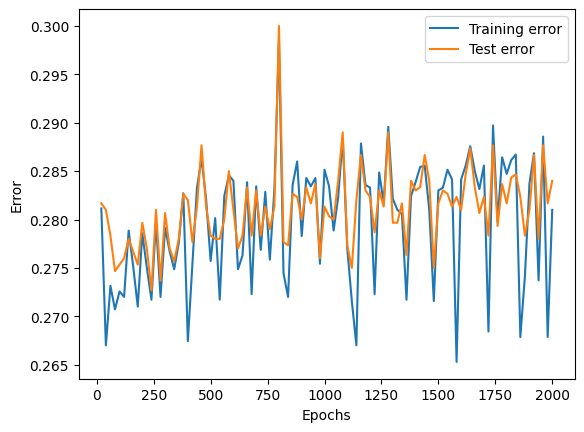
\includegraphics[width=0.8\columnwidth]{../plots/perceptron.png}
	\caption{Training and test errors of the perceptron depending on the number of epochs}
	\label{fig:perceptron}
\end{figure}

Figure \ref{fig:perceptron} show performances of perceptron aglorithm on the training and test set, based on the number of epochs. The errors on both sets are quite stable around 0.28, but it shows slightly better predictions on the very early epochs, while the error increases with the number of epochs. Looking at this results, the dataset is probably non linearly separable, as the algorithm didn't converge during the experiments and the error floats around the same values.

\paragraph{Quadratic feature extraction}
We try to improve the quality of predictions applying quadratic feature extraction, at the cost of a computationally more intensive predictor: starting from 11 feature, the quadratic feature extraction generate data points of 66 features. 
Figure \ref{fig:quad_perceptron} shows the achieved errors. In this case, despite certain spikes, the relationship between epochs and error is more evident, but it's also visible how increasing the number of epochs after a certain point brings the model to be less stable.

\begin{figure}
	\centering
	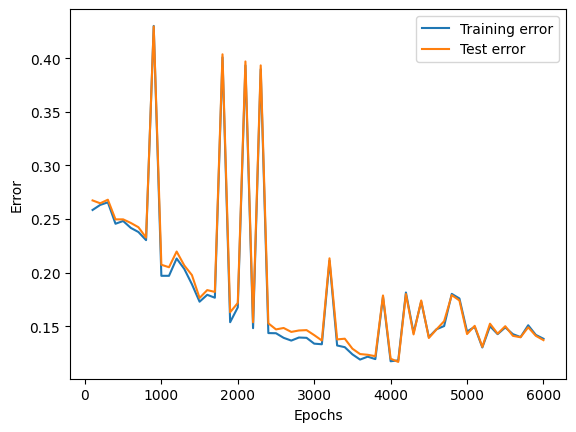
\includegraphics[width=0.8\columnwidth]{../plots/quad_perceptron.png}
	\caption{Training and test errors of the perceptron with quadratic feature extraction depending on the number of epochs}
	\label{fig:quad_perceptron}
\end{figure}

\paragraph{Kernel trick}
There's room for improvement by applying a polynomial extraction of higher degree, although the training tends to be computationally intractable even for relatively small degrees and training set, as the number of features explodes even with a relatively small degree: considering 10 features, with a degree of 3, the number of features would be 286, while with degree set to 4 the number of features would be 1001.

Kernel methods can be used to overcome this problem.
...
...

\begin{figure}
	\centering
	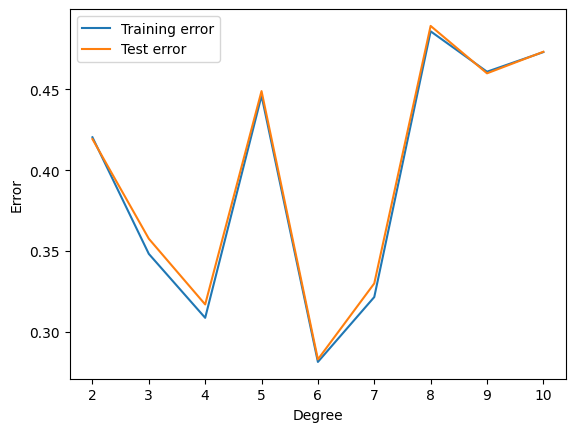
\includegraphics[width=0.8\columnwidth]{../plots/kpoly_perceptron.png}
	\caption{Training and test errors of the perceptron with quadratic feature extraction depending on the number of epochs}
	\label{fig:kpoly_perceptron}
\end{figure}




\end{document}